\documentclass[12pt]{paperFormatting}
% TikZ libraries needed for positioning and ellipse nodes
\usetikzlibrary{positioning,shapes.geometric,arrows.meta,fit}
\usepackage{fancyvrb}
% \usepackage{amsmath, amssymb, amsthm, graphicx, tikz, hyperref}
% \usepackage{bm}
% \usepackage{mathrsfs}

% \title{Meet The Flockers:\\ First Principles of Emergent Stratagem\\ in Next-Generation, Adversarial\\ Drone Warfare}
\title{When\\ \textit{Meeting The Flockers}\\\textit{Sleeps With The Fishes}:\\ First Principles of Emergent Stratagem\\ in Next-Generation, Adversarial\\ Drone Warfare}
\author{Jordan Jiosi} 
\copyrightyear{2025}
\academicyear{2025}

\begin{document}
\makeTitlePage

\begin{abstract}
Autonomous dominance across air and sea, spanning swarms, single-vehicle copilots for Gen-5/6 aerial fighters, or escorts for seafaring combat strike groups, requires control architectures that are tractable, robust, and verifiable under adversarial pressure. I show that standard reinforcement learning (RL), even with TRPO/PPO/MADDPG/MA-AIRL/GRPO, remains structurally tethered to its own sampling distributions, incurring variance, brittleness, and poor extrapolation in multi-agent combat where policies co-evolve. \\

As a transformational alternative, I derive a mean-field program that replaces policy-centric updates with physics-level equations of motion. In the large-population limit, agent collectives admit effective stochastic dynamics; extending to Dynamical Mean-Field Theory (DMFT) yields self-consistent memory kernels and colored noise that capture long-range temporal dependence and shock propagation (e.g., jamming, locks, decoys). \\

Crucially, I unify \emph{aerial murmurations} and \emph{aquatic schooling}: fish introduce hydrodynamic \emph{memory} (vortex wake) that naturally fits the DMFT kernel formalism, providing a direct bridge from bait-ball defenses and toroidal collapses to \emph{aerial acrobatics} and deception maneuvers. \\

This departure from a traditional RL paradigm preserves data efficiency and adds interpretability through response operators, enabling principled safety envelopes and real-time fault isolation for distributed swarms, AI aerial copilots on crewed Gen-5/6 aircraft, or AI seafaring escorts to crewed naval combat strike groups, and future \emph{multi-role, combined air-sea, shapeshifting transformers}.

This work contributes three novel elements:
\begin{enumerate}
  \item \textbf{Paradigm exit from RL to Mean-Field/DMFT.} We demonstrate RL's structural limits (distributional tethering, high variance, local exploration) and replace distribution-bound updates with Mean-Field Theory (MFT) and its dynamical extension, DMFT.
    \subitem{\emph{Why it matters:} yields scalable, closed-form dynamics that can be stress-tested and audited in advance, unlike distribution-tied RL rollouts; provides certifiable behavior for both swarms and single-aircraft copilots.}
  \item \textbf{DMFT with self-consistent kernels.} We extend DMFT with memory kernels and colored noise to model temporal propagation and adversarial perturbations.
  \subitem{ \emph{Why it matters:} predicts and hardens responses to shocks such as jamming, missile locks, decoys, or evasive maneuvers; supports rapid, linear-response re-tasking and principled fault isolation in real time.}
  \item \textbf{Elliptic-curve murmuration as algebraic topology.} We link Frobenius-trace distributions over finite fields to DMFT, furnishing cryptographically grounded, structured interaction graphs and routing schemes.
  \subitem{\emph{Why it matters:} enables cohesive (biomimetic) and defensive motion—denial walls, escort behaviors while maintaining secure coordination under electronic warfare; applicable to inter-vehicle swarms and intra-aircraft sensor/actuator fabrics for copilots.}
\end{enumerate}

Together, these advances yield a unified and auditable stack: \\
Stochastic Agent Dynamics $\to$ MFT $\to$ DMFT $\to$ Mean-Field Games $\to$ Control \\
that supports tractable, interpretable, and secure autonomy across modalities. Conceptual diagrams and first-principles derivations ground the framework; hardware-in-the-loop studies outline airspace denial walls, resilient escort behaviors, murmuration-style deception, bait-ball inspired \emph{toroidal/shield} formations, and \emph{Gen-5/6 AI copilot} integration. Beyond aerospace defense, the approach suggests broader applications in complex adaptive systems, density-functional expansions, and quantum analogs.
\end{abstract}

\section{Introduction}

The uncanny coherence observed in starling murmurations has long inspired interdisciplinary research into emergent collective behavior. This thesis extends such biological insights to adversarial drone swarms by developing a rigorous, multi-layered theoretical framework. Beginning from stochastic agent models and Group Relative Policy Optimization (GRPO; an RL method); we also use a generalized response-to-perturbed-observables lens to connect dynamics and control, we derive Mean-Field (MF) and Dynamic Mean-Field Theory (DMFT) descriptions capturing temporal memory and non-Markovian effects. We further incorporate Mean-Field Game (MFG) theory to model strategic decision-making among competing agents, and Density Functional Theory (DFT) to characterize spatial-temporal distributions. 

A novel contribution is the integration of arithmetic murmuration concepts via elliptic curve aggregates, providing algebraic finite-field abstractions for interaction topologies. These enable modeling of encrypted communication channels and adversarial routing in swarm networks. By combining these perspectives, we propose a unified theoretical foundation for next-generation adversarial drone warfare, emphasizing local interactions, global coherence, and strategic adaptability.

The structure of this document is as follows: Section 2 reviews biological and arithmetic murmuration. Section 3 develops the stochastic agent dynamics model and Mean-Field limits. Section 4 extends to DMFT with memory kernels and signal propagation. Section 5 introduces elliptic curve murmuration and finite-field abstractions. Section 6 formulates Mean-Field Games and control-theoretic frameworks. Section 7 presents Density Functional expansions. Section 8 discusses applications to drone swarm combat scenarios, including simulation approaches. Section 9 concludes with expanded future directions.

\section{Biological and Arithmetic Murmuration}

\subsection{2.1 Biological Murmuration: Local Interaction and Coherence}

Starling murmurations exemplify emergent collective behavior arising from simple local interaction rules. Empirical studies \cite{ballerini2008interaction, cavagna2010scale} show that each bird aligns its velocity to approximately seven nearest neighbors, establishing a bounded locality that fosters spatial coherence without centralized control. Perturbations propagate as structured waves with characteristic decay lengths, enabling rapid information transfer across the flock.

Mathematically, this can be modeled as a system of stochastic differential equations (SDEs) for agent states $x_i(t)$, with interactions restricted to nearest neighbors:
\begin{equation}
\dot{x}_i = f\big(x_i, \{x_j : j \in \mathcal{N}_i\}\big) + \eta_i(t),
\end{equation}
where $\mathcal{N}_i$ denotes the set of neighbors of agent $i$, and $\eta_i(t)$ is noise.

\subsection{2.2 Arithmetic Murmuration: Elliptic Curve Aggregates}

Recent advances \cite{mazur2022elliptic, quanta2024murmuration} have uncovered an intriguing arithmetic analog of murmuration in the distribution of Frobenius traces of elliptic curves over prime fields. Unlike spatial locality, this "arithmetic locality" operates over finite prime windows, exhibiting coherence in rank and conductor distributions reminiscent of biological murmuration.

Consider a family of elliptic curves $E_p$ defined over finite fields $\mathbb{F}_p$ with Frobenius endomorphisms characterized by trace $a_p$. Statistical distributions of $a_p$ over intervals of primes reveal structured correlations analogous to local interactions:
\begin{equation}
\{a_p : p \in [P, P+W]\} \quad \text{with } W \ll P,
\end{equation}
where $W$ is a conductor window size.

This arithmetic murmuration suggests universality of coherence phenomena across Euclidean and algebraic domains, supporting the hypothesis that structured averaging underlies emergent flocking behavior.

\section{From Stochastic Agent Dynamics to Mean-Field Theory}
\label{sec:dynamics-mf}

\subsection{3.0 GRPO: Group Relative Policy Optimization (RL)}
\label{sec:grpo-rl}
We use GRPO in its reinforcement learning sense: a policy-gradient method that centers advantages by a group-relative baseline to reduce variance and induce cooperative/competitive shaping in multi-agent settings. For a joint policy \(\pi_\theta\), the objective \(J(\theta)=\mathbb{E}[R]\) yields the gradient
\begin{equation}
\nabla_\theta J(\theta) = \mathbb{E}_{\pi_\theta}\big[\nabla_\theta \log \pi_\theta(a\mid s)\, \hat A^{\text{group}}(s,a)\big],\qquad \hat A^{\text{group}}(s,a)=\hat R_i-\overline{R}_{\text{group}}.
\end{equation}
This sits in the RL/control layer (see Fig.~\ref{fig:concept-bridge}) alongside TRPO/PPO/MADDPG/MA-AIRL and informs the policy/control variable \(u_i\). The *response-to-perturbations* viewpoint later connects policy updates to effective dynamics via linear response.

\subsection{3.1 Agent-Based Stochastic Dynamics}

We model each drone or bird as a stochastic agent with internal state $x_i(t) \in \mathbb{R}^d$ evolving according to a generalized Langevin-type equation:
\begin{equation}
\dot{x}_i = -\frac{\partial H}{\partial x_i} + \eta_i(t),
\label{eq:grpo}
\end{equation}
where $H$ is the interaction Hamiltonian encoding agent couplings, and $\eta_i(t)$ is a stochastic noise term, potentially Gaussian, Cauchy, or adversarially generated.

The Generalized Response to Perturbed Observables (GRPO) formalism \cite{marconi2008fluctuation} captures the response of the system to perturbations, enabling analysis of stability and propagation of signals.

\subsection{3.2 Mean-Field Limit}

As the number of agents $N \to \infty$, individual fluctuations average out, and the system dynamics converge to a mean-field description:
\begin{equation}
\dot{x}_i = -V'(x_i) + J \langle x \rangle + \eta_i(t),
\label{eq:meanfield}
\end{equation}
where $V$ is a potential function, $J$ is a coupling constant, and $\langle x \rangle = \frac{1}{N} \sum_{j=1}^N x_j$ is the empirical mean field.

This limit neglects temporal correlations and memory effects, providing a first-order approximation of collective behavior.

\subsection{3.3 Finite-Field and $k$-Nearest Neighbor Abstractions}

To model spatially bounded interactions beyond Euclidean space, we place agents in finite fields $\mathbb{F}_q^d$ and define neighborhoods via algebraic closeness or $k$-nearest neighbor (knn) embeddings:
\begin{itemize}
  \item Agents are indexed by elements in $\mathbb{F}_q^d$.
  \item Neighborhood $\mathcal{N}_i = \{j : d_{\mathbb{F}_q}(i,j) \leq k\}$, where $d_{\mathbb{F}_q}$ is an algebraic metric.
\end{itemize}

This abstraction supports modeling of encrypted communication networks and adversarial routing topologies, extending biological murmuration principles to cyber-physical domains.

\section{Dynamic Mean-Field Theory and Signal Propagation}

\subsection{4.1 Dynamic Mean-Field Theory (DMFT)}

DMFT incorporates temporal memory and self-consistent noise statistics into the mean-field description. Using the cavity method \cite{georges1996dynamical}, the dynamics for agent $i$ satisfy:
\begin{equation}
\dot{x}_i(t) = -V'(x_i(t)) + \int_0^t \Gamma(t-s) x_i(s) ds + \xi_i(t),
\label{eq:dmft}
\end{equation}
where $\Gamma$ is a memory kernel encoding past interactions, and $\xi_i(t)$ is colored noise with statistics determined self-consistently by the ensemble.

The memory kernel captures retardation effects and signal propagation delays, essential for modeling real-time swarm responses.

\subsection{4.2 Signal Propagation in Weakly Coupled Systems}

Perturbations to a single agent induce ripple effects across neighbors. In biological flocks, a bird's turn generates a decaying wave of velocity changes. In DMFT, the memory kernel $\Gamma$ explicitly governs this propagation:
\begin{equation}
\delta x_i(t) = \int_0^t \Gamma(t-s) \delta x_j(s) ds + \cdots,
\end{equation}
with decay and dispersion characteristics determined by $\Gamma$.

This framework enables quantitative prediction of information flow and robustness to adversarial inputs such as jamming or targeted attacks.

%===============================
\section{Unified Control Without Bellman: Mean-Field SDEs, Memory Kernels, Response}
\label{sec:unified-nobellman}

\paragraph{Core objects (domain-agnostic).}
Let each agent have state $x_i(t)\in\mathbb{R}^d$ and control $u_i(t)$.
The stochastic microdynamics with memory are
\begin{equation}
\label{eq:mf-memory-sde}
dx_i(t)=\big[f(x_i,t)+u_i(t)\big]\,dt
+\int_0^t \Gamma(t-s)\,g\!\big(x_i(s)\big)\,ds\,dt
+\sigma\,dW_i(t),
\end{equation}
where $\Gamma(\cdot)$ is a \emph{memory kernel} (interaction+environment) and
$\sigma dW_i$ is colored noise realized by a filter consistent with the ensemble.

On the population level, the density $m(t,x)$ obeys a continuity/diffusion law
\begin{equation}
\label{eq:mf-continuity}
\partial_t m(t,x)=
-\nabla\!\cdot\!\Big(m\,\big[f(x,t)+u^\star(t,x)\big]\Big)
+\tfrac12\nabla\!\cdot\!\big(D\,\nabla m\big),\qquad D=\sigma\sigma^\top.
\end{equation}

Small exogenous perturbations $h$ (e.g.\ jamming, feints) drive observables $O$ via linear response:
\begin{equation}
\label{eq:kubo}
\delta\!\langle O\rangle(t)=\int_0^t \chi_O(t-s)\,\delta h(s)\,ds,\qquad
\chi_O(t)=\frac{d}{dh}\Big|_{h=0}\langle O\rangle_h(t).
\end{equation}

\paragraph{Control without dynamic programming.}
We select controls by minimizing a \emph{kernel-aware action} (no value function):
\begin{equation}
\label{eq:kernel-action}
\mathcal{J}[u]=\int_0^T\!\Big(
\underbrace{\Phi(m_t)}_{\text{formation/mission cost}}
+\underbrace{\tfrac12\,\|u\|_{\mathcal{K}^{-1}}^2}_{\text{effort in kernel metric}}
-\underbrace{\langle r_t,\,O(m_t)\rangle}_{\text{task drive}}
\Big)\,dt,\quad
\|u\|_{\mathcal{K}^{-1}}^2=\int u^\top \mathcal{K}^{-1} u\,dx,
\end{equation}
with $\mathcal{K}$ chosen from the same operator family as $\Gamma$.
Stationarity of $\mathcal{J}$ yields Euler-Lagrange conditions on $u^\star$ coupled to
\eqref{eq:mf-continuity}. \emph{Interpretation:} we steer the ensemble in the operator
basis that governs propagation, giving closed/semi-closed feedback without Bellman/RL.

\paragraph{Domain mapping (same math, different semantics).}
\begin{center}
\begin{tabular}{@{}l l l l l l@{}}
\toprule
Domain & State $x$ & Drift $f$ & Kernel $\Gamma$ / coupling & Control $u$ & Observable $O$\\
\midrule
Flocking & pose+heading & turn kinematics & 7-NN align + delay & heading/speed bias & cohesion $\Phi=\|\bar v\|$, wave speed\\
Fish bait balls & pose + local flow & advection + lift/drag & hydrodynamic wake (Biot-Savart/SL) & turn/radial bias & drag proxy, perimeter density \\
Aerial dogfights & pos/vel/LOS & kinematics+fusion & comms \& guidance delays & thrust/pitch/yaw bias & lock prob., miss distance \\
Infantry & pose+cover occupancy & terrain diffusion & LOS occlusion, morale & move/fire discipline & exposure, cross-fire index \\
BJJ/Boxing & distance, angle, posture & bio-mechanics & grip/clinching hysteresis & feint/grapple/hip shift & advantage, off-balancing \\
\bottomrule
\end{tabular}
\end{center}

\subsection{Fish Schooling as Hydrodynamic Memory}
\label{sec:fish-memory}
For fish, we decompose
\begin{equation}
\Gamma(t)=\Gamma_{\text{align}}(t)+\Gamma_{\text{wake}}(t),
\end{equation}
where $\Gamma_{\text{align}}$ captures social alignment and
$\Gamma_{\text{wake}}$ encodes delayed lift/drag from neighbors’ vortices.
In practice, $\Gamma_{\text{wake}}(t)\approx\sum_{k=1}^K a_k e^{-t/\tau_k}$ (few decaying modes fit to CFD/data).
Natural observables are perimeter density (bait-ball ``shell''), internal velocity variance (cohesion), and an energy/drag proxy.

\paragraph{Closed-form shapeshifting (biomimicry).}
Given a target formation field $m^\dagger(x,t)$ (e.g.\ torus $\to$ sheet $\to$ wedge),
\begin{equation}
\Phi(m_t)=\lambda_1\,\mathrm{KL}(m_t\Vert m^\dagger_t)+\lambda_2\,\|\mathcal{P}m_t\|^2,
\end{equation}
with $\mathcal{P}$ projecting out undesirable modes (e.g.\ radial buckling). The feedback that minimizes \eqref{eq:kernel-action} is
\begin{equation}
\label{eq:kernel-feedback}u^\star(t,x)=\mathcal{K}\,\nabla_x \Big(\delta\Phi/\delta m\Big)(t,x),
\end{equation}
i.e.\ push along the kernel’s easy directions—\emph{analytical, auditable, and fast}.
This implements our favored capability: \emph{shapeshifting murmurations} with closed-form biomimicry.

\subsection{Implementation Skeleton (No Bellman, No RL)}
\vspace{-0.25em}
\begin{Verbatim}[fontsize=\small, frame=single, samepage=true]
# 1) Estimate kernel Gamma and colored-noise stats from data or micro-sim
Gamma, C_xi = fit_kernel_and_noise(tracks, topology="7NN" 
                                                  or "hydro" 
                                                  or "EC-graph")

# 2) Define ensemble cost Phi and operator metric K (from Gamma)
def formation_cost(m, t):
    return KL(m, target_density(t)) + lambda2 * norm(P(m))**2

# 3) Continuity step: d/dt m = -div(m*(f+u)) + 1/2 * div(D * grad m)
def step_density(m, u, dt):
    return advect_diffuse(m, drift=f_field, control=u, D=D, dt=dt)

# 4) Control law in kernel metric: u* = K * grad(dPhi/dm)
def feedback_control(m, t):
    grad = variational_derivative(formation_cost, m, t)
    return apply_kernel_metric(K_from(Gamma), grad)

# 5) Closed-loop shapeshifting
m = init_density()
for t in time_grid:
    u = feedback_control(m, t)
    m = step_density(m, u, dt)
    # optional: inject colored noise consistent with C_xi
\end{Verbatim}
\vspace{-0.5em}

\paragraph{Operational note.}
The same controller \eqref{eq:kernel-feedback} applies to birds, fish, drones, infantry—only the meanings of $f,\Gamma,O$ change. 
Aquatic ``acrobatics'' and toroidal bait-ball strategies transfer to \emph{aerial acrobatics} by swapping $\Gamma_{\text{wake}}$ for aerodynamic delay kernels and reinterpreting $O$ as lock-probability, miss-distance, or EW-resilience indices.
%===============================

\section{Elliptic Curve Murmuration and Finite-Field Topologies}

\subsection{5.1 Algebraic Interaction Networks}

Inspired by arithmetic murmuration, we define interaction graphs based on elliptic curve aggregates over finite fields. Let $\mathbb{F}_q$ be a finite field of order $q$, and consider elliptic curves $E/\mathbb{F}_q$ with group structure $E(\mathbb{F}_q)$.

Agents correspond to points on $E(\mathbb{F}_q)$, and neighborhoods are defined via group operations or conductor windows:
\begin{equation}
\mathcal{N}_P = \{Q \in E(\mathbb{F}_q) : \text{dist}(P,Q) \leq k\},
\end{equation}
where $\text{dist}$ is an algebraic metric, e.g., number of additions needed to reach $Q$ from $P$.

\subsection{5.2 Coherence via Frobenius Trace Distributions}

The Frobenius endomorphism $\pi$ acts on $E(\mathbb{F}_q)$ with trace $a_q = q + 1 - |E(\mathbb{F}_q)|$. Statistical distributions of $a_q$ over prime windows exhibit coherence analogous to velocity alignment in flocks.

This arithmetic coherence supports secure, structured communication protocols for swarms operating in adversarial environments, leveraging cryptographic hardness assumptions.

\section{Mean-Field Games and Control Theory}

\subsection{6.1 Mean-Field Game Formulation}

Mean-Field Games \cite{lasry2007mean, huang2006large} model strategic interactions among a large population of rational agents. Each agent $i$ controls state $x_i(t)$ to minimize a cost functional:
\begin{equation}
J_i = \mathbb{E} \left[ \int_0^T L(x_i(t), u_i(t), m_t) dt + g(x_i(T), m_T) \right],
\end{equation}
where $u_i(t)$ is the control, $m_t$ is the distribution of states at time $t$, $L$ is a running cost, and $g$ is a terminal cost.

The coupled Hamilton-Jacobi-Bellman (HJB) and Fokker-Planck (FP) equations characterize the equilibrium:
\begin{align}
-\partial_t V(t,x) &= \min_u \left\{ L(x,u,m_t) + \nabla V \cdot f(x,u) + \frac{1}{2} \text{Tr}(\sigma \sigma^T \nabla^2 V) \right\}, \\
\partial_t m_t &= - \nabla \cdot (m_t f(x,u^*)) + \frac{1}{2} \nabla^2 : (m_t \sigma \sigma^T),
\end{align}
where $V$ is the value function, and $u^*$ is the optimal control.

\subsection{6.2 Control-Theoretic Extensions}

In adversarial drone swarms, agents optimize trajectories balancing objectives such as engagement, evasion, and communication. Control inputs $u_i$ influence states $x_i$ evolving under stochastic dynamics:
\begin{equation}
dx_i = f(x_i,u_i) dt + \sigma dW_t,
\end{equation}
with $W_t$ a Wiener process.

Using MFG, we derive decentralized control policies robust to adversarial perturbations, enabling emergent cooperative or competitive stratagems.

\section{Density Functional Extensions}

\subsection{7.1 Density Functional Theory for Agent Distributions}

Extending Mean-Field formulations, Density Functional Theory (DFT) \cite{evans1979nature} models the free energy $\mathcal{F}[m]$ as a functional of agent density $m(x,t)$:
\begin{equation}
\mathcal{F}[m] = \mathcal{F}_{\mathrm{id}}[m] + \mathcal{F}_{\mathrm{ex}}[m],
\end{equation}
where $\mathcal{F}_{\mathrm{id}}$ is the ideal gas contribution and $\mathcal{F}_{\mathrm{ex}}$ encodes interactions.

The equilibrium density minimizes $\mathcal{F}[m]$ subject to constraints:
\begin{equation}
\frac{\delta \mathcal{F}}{\delta m(x)} = \mu,
\end{equation}
with $\mu$ a chemical potential.

\subsection{7.2 Dynamic Density Functional Theory (DDFT)}

DDFT extends DFT to time-dependent densities $m(x,t)$ satisfying a continuity equation with fluxes driven by functional derivatives of $\mathcal{F}$:
\begin{equation}
\partial_t m(x,t) = \nabla \cdot \left( m(x,t) \nabla \frac{\delta \mathcal{F}}{\delta m(x,t)} \right).
\end{equation}

This framework models spatiotemporal evolution of agent distributions, capturing clustering, dispersion, and wave-like propagation in swarms.

\section{Applications: Adversarial Drone Swarms}

\subsection{8.1 Simulation of DMFT-Driven Drone Swarms}

Using the DMFT framework with memory kernels and colored noise, we simulate drone swarms engaged in adversarial combat. Agents follow stochastic dynamics with control inputs derived from MFG solutions.

\subsection{8.2 Tactical Scenarios}

\begin{itemize}
  \item \textbf{Airspace Denial Walls:} Defensive drones form dynamic barriers using local interaction rules to prevent enemy incursions.
  \item \textbf{Murmuration-Inspired Confusion:} Adversarial swarms mimic natural murmuration patterns to disrupt targeting algorithms.
  \item \textbf{Response Functions:} Derived from DMFT memory kernels, enabling rapid adaptation to missile locks, jamming, and evasion.
\end{itemize}

\subsection{8.3 Conceptual Diagram of Multi-Layered Framework}

\begin{figure}[H]
\centering
\resizebox{\linewidth}{!}{%
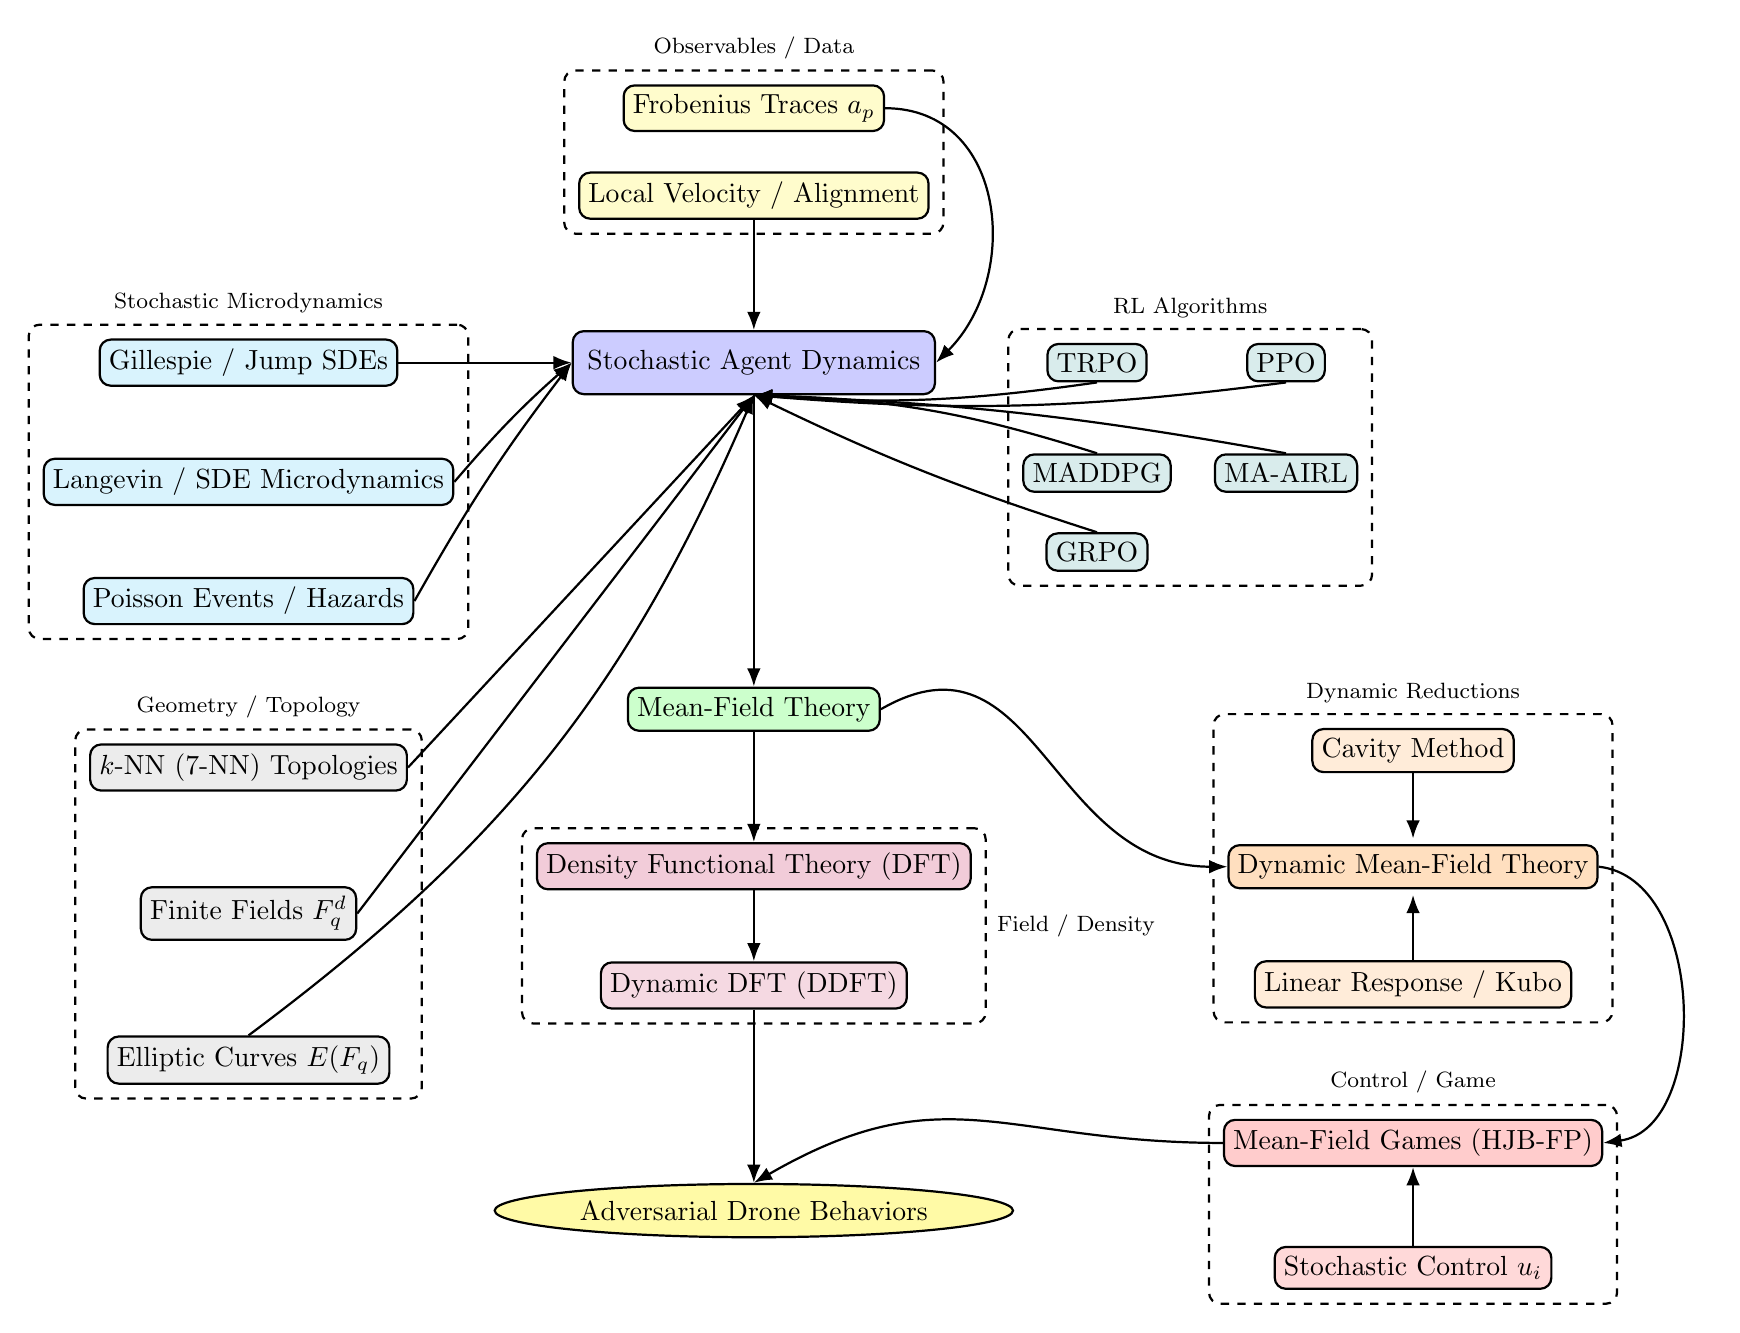
\begin{tikzpicture}[node distance=1.4cm and 2.1cm, auto, thick, every node/.style={transform shape}, >=Latex]
  % Core node
  \node[draw, rectangle, rounded corners, fill=blue!20, minimum width=46mm, minimum height=8mm] (DYN) {Stochastic Agent Dynamics};

  % Families feeding into GRPO -------------------------------------------------
  % Stochastic microdynamics family (upper-left)
  \node[draw, rectangle, rounded corners, fill=cyan!15, left=1.4cm and 2.2cm of DYN] (Gillespie) {Gillespie / Jump SDEs};
  \node[draw, rectangle, rounded corners, fill=cyan!15, below=0.9cm of Gillespie] (Langevin) {Langevin / SDE Microdynamics};
  \node[draw, rectangle, rounded corners, fill=cyan!15, below=0.9cm of Langevin] (Poisson) {Poisson Events / Hazards};
  % Group box for stochastic microdynamics
  \node[draw, dashed, rounded corners, inner sep=5pt, fit=(Gillespie)(Langevin)(Poisson), label=above:{\footnotesize Stochastic Microdynamics}] (BoxMicro) {};

  % RL algorithms family (upper-right)
  \node[draw, rectangle, rounded corners, fill=teal!15, right=1.4cm of DYN] (TRPO) {TRPO};
  \node[draw, rectangle, rounded corners, fill=teal!15, right=1.25cm of TRPO] (PPO) {PPO};
  \node[draw, rectangle, rounded corners, fill=teal!15, below=0.9cm of TRPO] (MADDPG) {MADDPG};
  \node[draw, rectangle, rounded corners, fill=teal!15, below=0.9cm of PPO] (MAAIRL) {MA-AIRL};
  \node[draw, rectangle, rounded corners, fill=teal!15, below=0.5cm of MADDPG] (GRPO) {GRPO};
  % Group box for RL algorithms
  \node[draw, dashed, rounded corners, inner sep=5pt, fit=(TRPO)(PPO)(MADDPG)(MAAIRL)(GRPO), label=above:{\footnotesize RL Algorithms}] (BoxRL) {};

  % Geometry / topology family (left)
  \node[draw, rectangle, rounded corners, fill=gray!15, below=1.5cm of Poisson] (kNN) {$k$-NN (7-NN) Topologies};
  \node[draw, rectangle, rounded corners, fill=gray!15, below=1.2cm of kNN] (Fq) {Finite Fields $\mathbb{F}_q^d$};
  \node[draw, rectangle, rounded corners, fill=gray!15, below=1.2cm of Fq] (Elliptic) {Elliptic Curves $E(\mathbb{F}_q)$};
  \node[draw, dashed, rounded corners, inner sep=5pt, fit=(kNN)(Fq)(Elliptic), label=above:{\footnotesize Geometry / Topology}] (BoxGeom) {};

  % Observables / data family (upper)
  \node[draw, rectangle, rounded corners, fill=yellow!20, above=1.4cm of DYN] (ObsVel) {Local Velocity / Alignment};
  \node[draw, rectangle, rounded corners, fill=yellow!20, above=0.5cm of ObsVel] (ObsFrob) {Frobenius Traces $a_p$};
  \node[draw, dashed, rounded corners, inner sep=5pt, fit=(ObsVel)(ObsFrob), label=above:{\footnotesize Observables / Data}] (BoxObs) {};

  % Edges into GRPO
  \draw[->] (Gillespie.east) -- (DYN.west);
  \draw[->, bend left=4] (Langevin.east) to (DYN.west);
  \draw[->, bend left=4] (Poisson.east) to (DYN.west);
  \draw[->, bend left=6]  (TRPO.south)   to (DYN.south);
  \draw[->, bend left=6]   (PPO.south)    to (DYN.south);
  \draw[->, bend right=8] (MADDPG.north) to (DYN.south);
  \draw[->, bend right=4] (MAAIRL.north) to (DYN.south);
  \draw[->, bend left=4] (GRPO.north) to (DYN.south);
  \draw[->] (kNN.east) to (DYN.south);
  \draw[->] (Fq.east) to (DYN.south);
  \draw[->, bend right=15] (Elliptic.north) to (DYN.south);
  \draw[->] (ObsVel.south) -- (DYN.north);
  \draw[->, in=45, out=360, looseness=1.2] (ObsFrob.east) to (DYN.east);
  % Downstream chain -----------------------------------------------------------
  \node[draw, rectangle, rounded corners, fill=green!20, below=3.7cm of DYN] (MF) {Mean-Field Theory};
  
  % Dynamic reductions family near DMFT
  \node[draw, rectangle, rounded corners, fill=orange!25, below right=5.7cm and 3.7cm of DYN] (DMFT) {Dynamic Mean-Field Theory};
  \node[draw, rectangle, rounded corners, fill=orange!15, above=0.9cm of DMFT] (Cavity) {Cavity Method};
  \node[draw, rectangle, rounded corners, fill=orange!15, below=0.9cm of DMFT] (Kubo) {Linear Response / Kubo};
  \node[draw, dashed, rounded corners, inner sep=5pt, fit=(Cavity)(DMFT)(Kubo), label=above:{\footnotesize Dynamic Reductions}] (BoxDyn) {};
  
  % Control family near MFG
  \node[draw, rectangle, rounded corners, fill=red!20, below=1.4cm of Kubo] (MFG) {Mean-Field Games (HJB-FP)};
  \node[draw, rectangle, rounded corners, fill=red!15, below=1.0cm of MFG] (POLICY) {Stochastic Control $u_i$};
  \node[draw, dashed, rounded corners, inner sep=5pt, fit=(MFG)(POLICY), label=above:{\footnotesize Control / Game}] (BoxCtrl) {};

  \node[draw, rectangle, rounded corners, fill=purple!20, below=1.4cm of MF] (DFT) {Density Functional Theory (DFT)};
  \node[draw, rectangle, rounded corners, fill=purple!15, below=0.9cm of DFT] (DDFT) {Dynamic DFT (DDFT)};
  \node[draw, dashed, rounded corners, inner sep=5pt, fit=(DFT)(DDFT), label=right:{\footnotesize Field / Density}] (BoxDens) {};

  % Applications (bottom)
  \node[draw, ellipse, fill=yellow!35, below=2.2cm of DDFT] (Applications) {Adversarial Drone Behaviors};

  % Chain arrows
  \draw[->] (DYN) -- (MF);
  \draw[->, in=180, out=30, looseness=1.2] (MF.east) to (DMFT.west);
  \draw[->] (POLICY) -- (MFG);
  \draw[->, bend left=83] (DMFT.east) to (MFG.east);
  \draw[->] (MF) -- (DFT);
  \draw[->] (DFT) -- (DDFT);
  \draw[->, out=180, in=30, looseness=1.2] (MFG.west) to (Applications.north);
  \draw[->] (DDFT.south) -- (Applications.north);

  % Optional supportive arrows
  \draw[->, shorten >=2pt] (Cavity) -- (DMFT);
  \draw[->, shorten >=2pt] (Kubo) -- (DMFT);
\end{tikzpicture}
}
\end{figure}

\section{Conclusion and Future Directions}

This thesis has developed a comprehensive, multi-disciplinary framework for modeling and controlling adversarial drone swarms, grounded in first principles of stochastic agent dynamics, mean-field theories, game theory, and algebraic abstractions. By integrating biological and arithmetic murmuration concepts, we have proposed novel finite-field interaction topologies and cryptographically inspired swarm protocols. The incorporation of dynamic memory kernels and control-theoretic formulations enables realistic modeling of signal propagation and strategic decision-making in adversarial environments.

Future research directions include:

\begin{itemize}
  \item \textbf{Quantum Analogs:} Extending DMFT and MFG frameworks to quantum many-body systems for quantum swarm control and quantum-secure communications.
  \item \textbf{Cryptographic Network Implementations:} Realizing elliptic curve murmuration-based protocols in hardware and software for secure drone swarm coordination.
  \item \textbf{Hardware-in-the-Loop Simulations:} Integrating theoretical models with real-world drone platforms and sensor networks for validation and refinement.
  \item \textbf{Policy and Ethical Implications:} Investigating regulatory frameworks, ethical considerations, and defense policy impacts of autonomous adversarial drone systems.
\end{itemize}

The synergy of physics, mathematics, computer science, and engineering presented herein lays a foundation for next-generation aerospace defense technologies and advances the scientific understanding of complex adaptive systems.

\appendix

\section*{Appendix A: Simulation Results}
\textit{Results from Gillespie-style stochastic simulations and DMFT-based numerical solvers are available upon request. Visualizations illustrating wave propagation, memory kernel effects, and strategic swarm maneuvers will be embedded in the final thesis PDF.}

\buildBibliography

\section*{Appendix B: Notation Table}

\begin{tabular}{ll}
$\Gamma(t)$ & Memory kernel governing temporal interactions \\
$\xi_i(t)$ & Self-consistent colored noise for agent $i$ \\
$x_i(t)$ & Internal state vector of agent $i$ at time $t$ \\
$k$ & Number of nearest neighbors in spatial or algebraic metric \\
$\mathbb{F}_q$ & Finite field of order $q$ \\
$E(\mathbb{F}_q)$ & Group of points of an elliptic curve over $\mathbb{F}_q$ \\
$m_t$ & Distribution of agent states at time $t$ \\
$u_i(t)$ & Control input for agent $i$ at time $t$ \\
$V$ & Potential function or value function, context dependent \\
$H$ & Hamiltonian encoding agent interactions \\
$J$ & Coupling constant in mean-field models \\
$\mathcal{F}[m]$ & Free energy functional of agent density $m$ \\
$W_t$ & Standard Wiener process (Brownian motion) \\
\end{tabular}

\end{document}
